\section{PROCEDIMIENTO} 

\begin{itemize}
\subsection{ Habriendo  Docker}
	\item Abrir el menu inicio y buscar la aplicación Docker for Windows.

	\item Ubicar la aplicación PowerShell(ejecutarla como Administrador). En la ventana de comandos de PowerShell escribir
lo siguiente.
		\begin{figure}[H]
		\begin{center}
		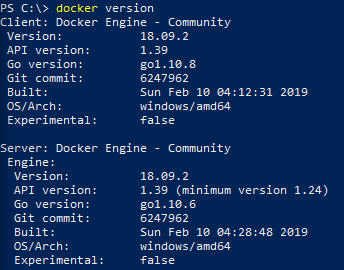
\includegraphics[width=8cm]{./Imagenes/1}
		\end{center}
		\end{figure}
     
\subsection{ Creando un contenedor con Oracle Database para Linux}
	\item Entrar a esete link (https://hub.docker.com/ )y Iniciar sesión o crear una cuenta nueva.
	\item Luego buscar  el repositorio para Oracle Database.Darle click en proceeed to  CheckOut, completar los datos y aceptar las condiciones obligatorias para obtener el acceso al contenido.
		\begin{figure}[H]
		\begin{center}
		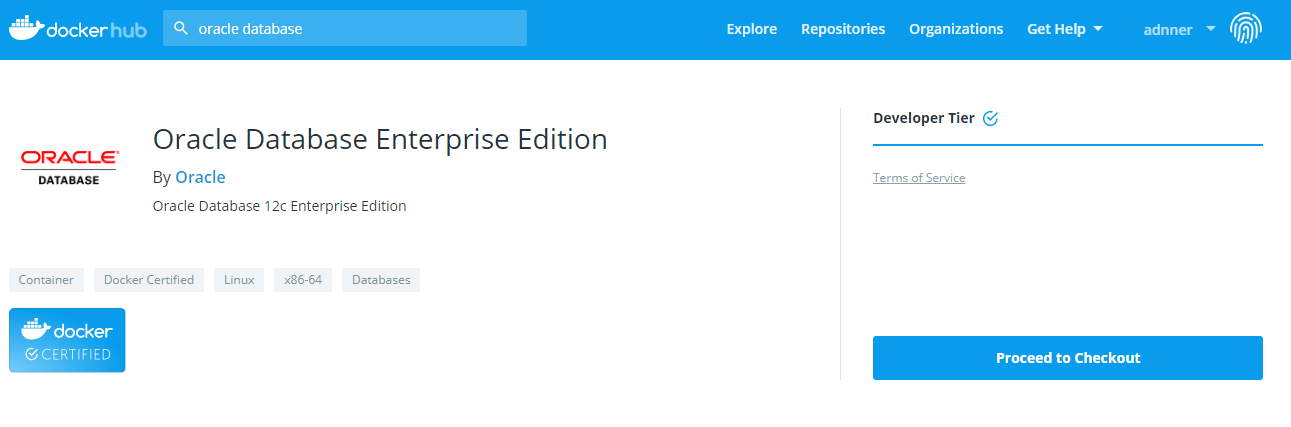
\includegraphics[width=8cm]{./Imagenes/3}
		\end{center}
		\end{figure}
	\item En la ventana de PowerShelql, escribir el siguiente comando:
		\begin{figure}[H]
		\begin{center}
		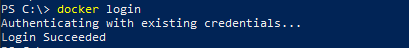
\includegraphics[width=9cm]{./Imagenes/4}
		\end{center}
		\end{figure}
	\item Ejecutar el siguiente comando en Powershell, lo cual descargará la imagen del contenedor de Oracle Database en un servidor Linux y nos pedirra talves nuestra cuenta en docker entonces se loguea 
		\begin{figure}[H]
		\begin{center}
		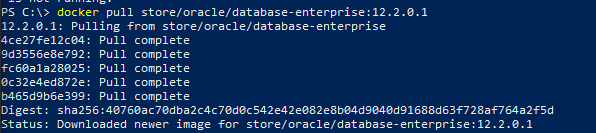
\includegraphics[width=15cm]{./Imagenes/5}
		\end{center}
		\end{figure}
	\item No aparecera como  respuesta  un ID que corresponde al contenedor.
		\begin{figure}[H]
		\begin{center}
		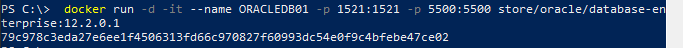
\includegraphics[width=15cm]{./Imagenes/6}
		\end{center}
		\end{figure}
	\item Verificar que el contenedor se esté ejecutando correctamente mediante el comando que ingresamos :
		\begin{figure}[H]
		\begin{center}
		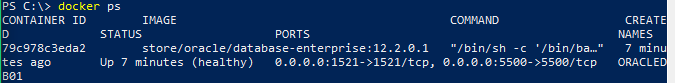
\includegraphics[width=15cm]{./Imagenes/7}
		\end{center}
		\end{figure}
	\item Cuando el estado del contenedor sea “healthy”, en la consola de Powershell, ejecutar el siguiente comando:
		\begin{figure}[H]
		\begin{center}
		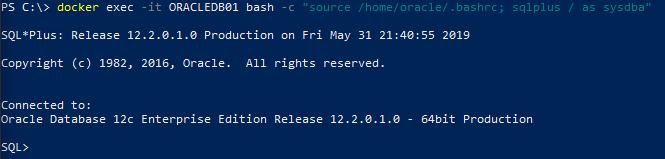
\includegraphics[width=15cm]{./Imagenes/8}
		\end{center}
		\end{figure}
	\item En la línea de comentados de SQL*Plus, escribir lo siguiente
		\begin{figure}[H]
		\begin{center}
		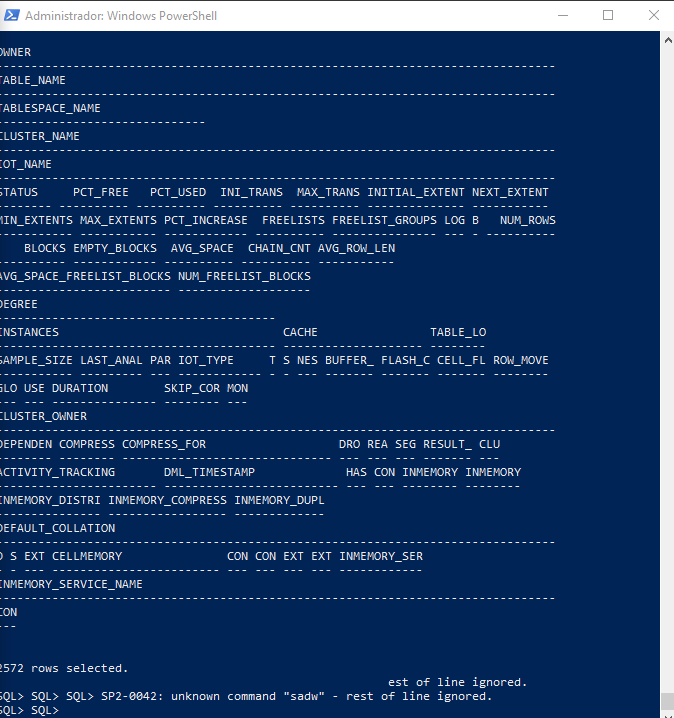
\includegraphics[width=8cm]{./Imagenes/19}
		\end{center}
		\end{figure}
	\item Escribir el comando quit para cerrar la sesión de SQL*Plus
		\begin{figure}[H]
		\begin{center}
		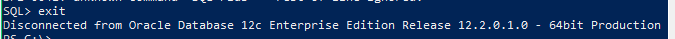
\includegraphics[width=15cm]{./Imagenes/10}
		\end{center}
		\end{figure}
	\item Ingresar a este link :https://localhost:5500/em. Iniciar sesión con los siguientes datos:
		\begin{figure}[H]
		\begin{center}
		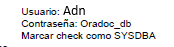
\includegraphics[width=4cm]{./Imagenes/t1}
		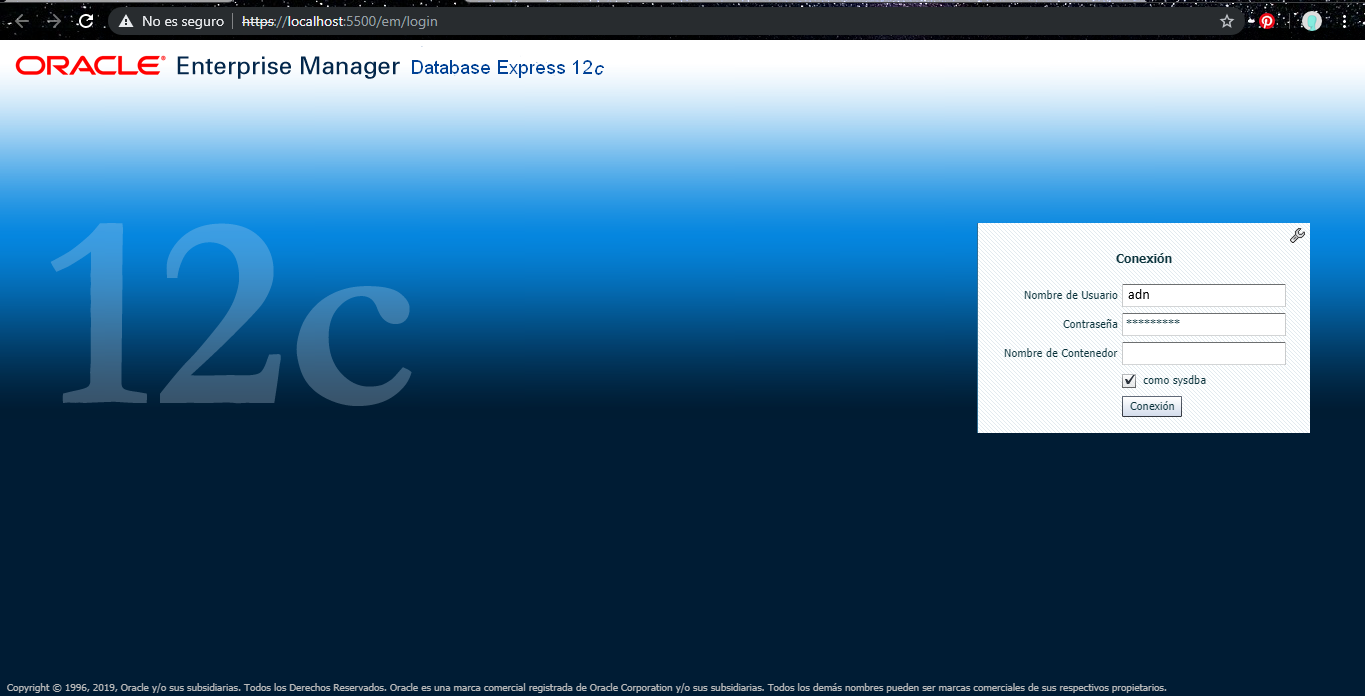
\includegraphics[width=15cm]{./Imagenes/11}
		\end{center}
		\end{figure}
	\item Luego se visualizará la siguiente ventana. Cerrar sesión y la pestaña del navegador de internet.
		\begin{figure}[H]
		\begin{center}
		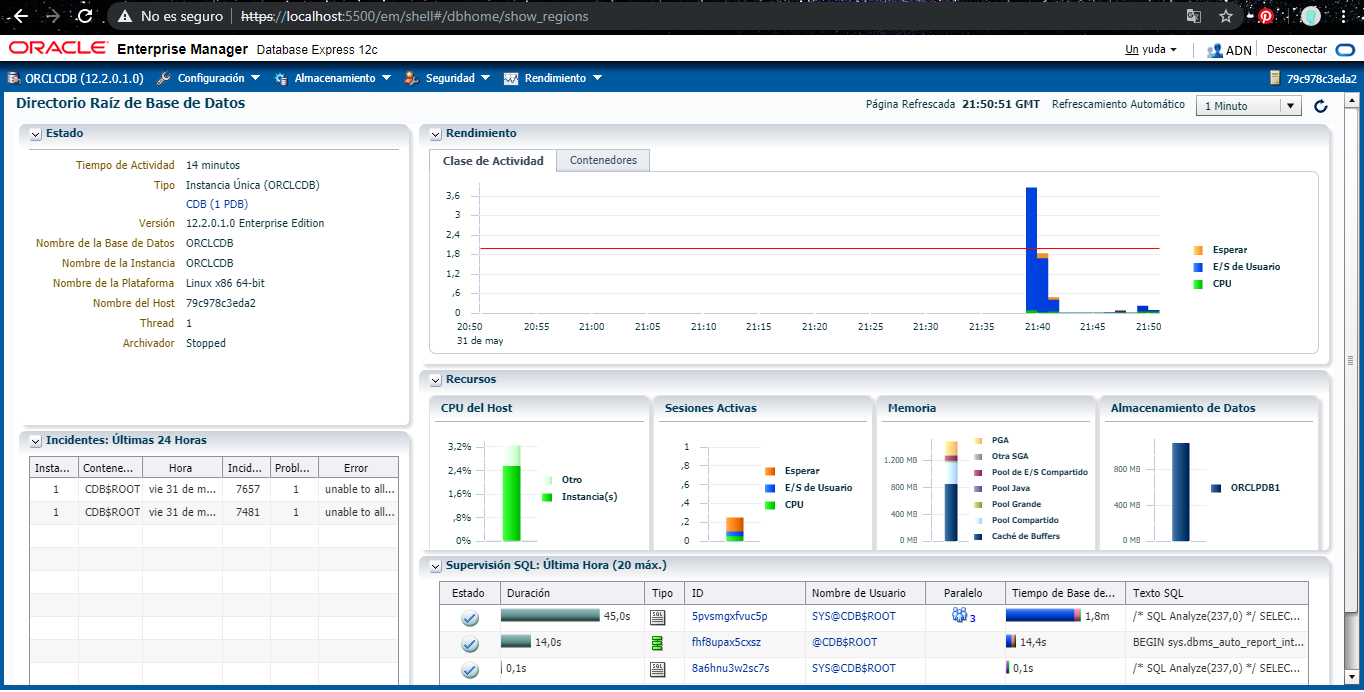
\includegraphics[width=15cm]{./Imagenes/12}
		\end{center}
		\end{figure}
	\item Iniciar el aplicativo Oracle SQL Developer y crear una nueva conexión con los siguientes parámetros:
		\begin{figure}[H]
		\begin{center}
		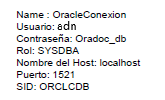
\includegraphics[width=5cm]{./Imagenes/t2}
		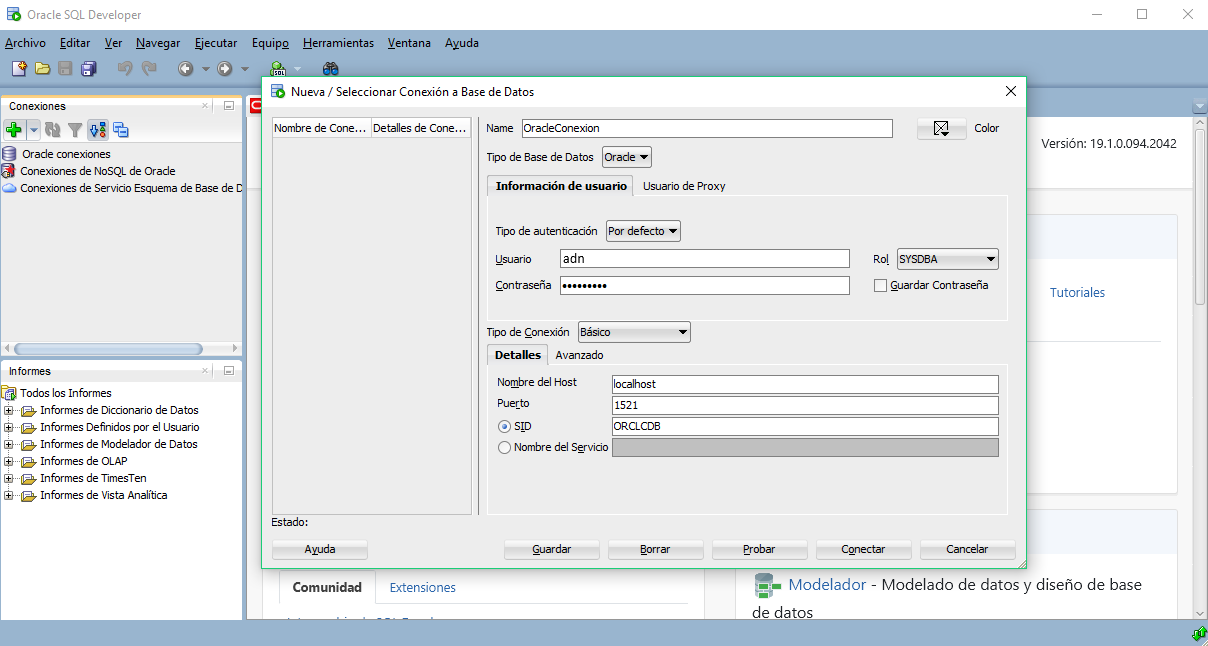
\includegraphics[width=15cm]{./Imagenes/13}
		\end{center}
		\end{figure}
	\item Damos una  nueva consulta, escribir y ejecutar lo siguiente; deberá retornar varios registros que representan las tablas de las base de datos
		\begin{figure}[H]
		\begin{center}
		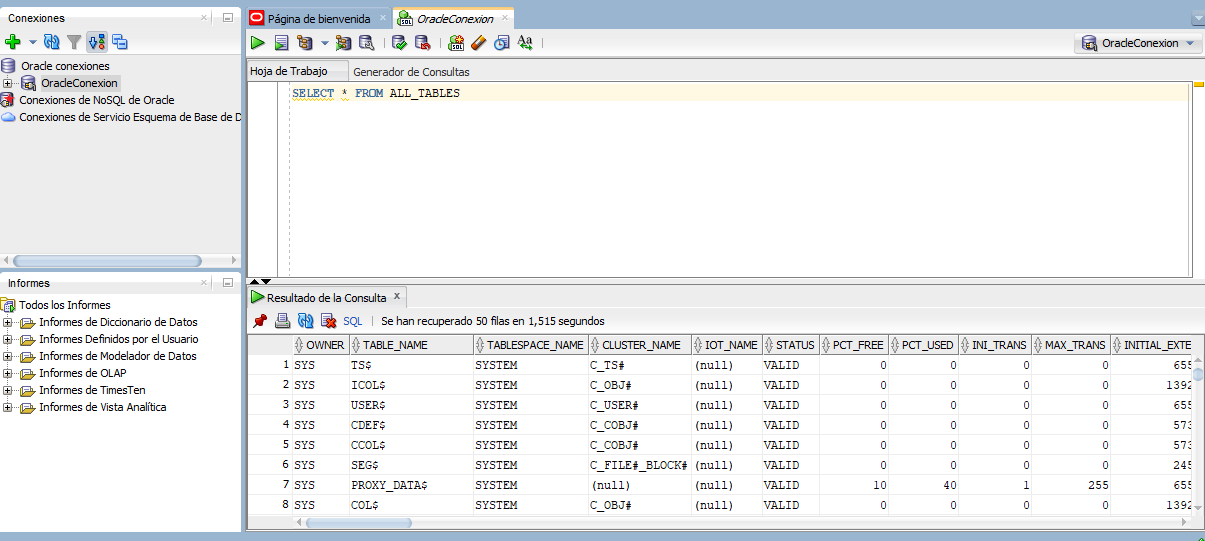
\includegraphics[width=15cm]{./Imagenes/14}
		\end{center}
		\end{figure}
	\item Cerrar la aplicación Oracle SQL Developer
	\item En PowerShell ejecutar el siguiente comando. Y verificar la eliminación del contenedor con ejecutando
		\begin{figure}[H]
		\begin{center}
		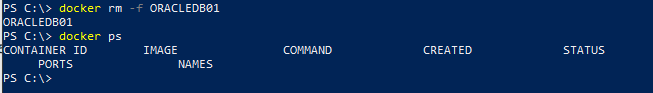
\includegraphics[width=12cm]{./Imagenes/15}
		\end{center}
		\end{figure}


\subsection{ Adicionando persistencia}
	\item En PowerShell ejecutar el siguiente comando, lo cual dara como respuesta se visualizará un ID que corresponde al contenedor
		\begin{figure}[H]
		\begin{center}
		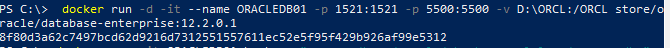
\includegraphics[width=12cm]{./Imagenes/16}
		\end{center}
		\end{figure}
	\item Repetir el paso 13 y modificar la contraseña del usuario SYS
		\begin{figure}[H]
		\begin{center}
		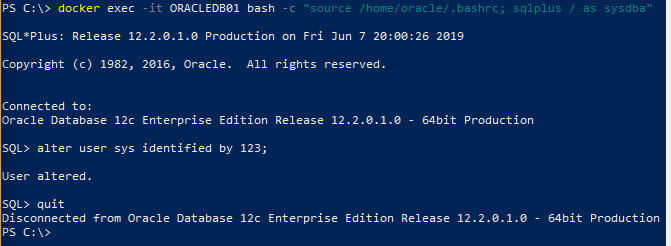
\includegraphics[width=12cm]{./Imagenes/20}
		\end{center}
		\end{figure}
       	\item Iniciar el aplicativo Oracle SQL Developer, conectarse como el usuario SYS y ejecutar el siguiente comando
		\begin{figure}[H]
		\begin{center}
		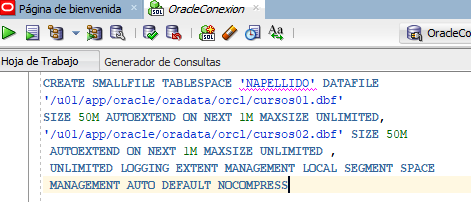
\includegraphics[width=12cm]{./Imagenes/22}
		\end{center}
		\end{figure}
	\item Verificar el contenido de la carpeta ORCL
	\item En PowerShell ejecutar el siguiente comando. Verificar la eliminación del contenedor con ejecutando
		\begin{figure}[H]
		\begin{center}
		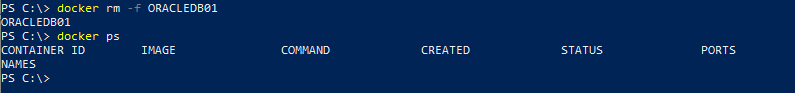
\includegraphics[width=12cm]{./Imagenes/24}
		\end{center}
		\end{figure}
	\item Cerrarmos  la aplicación Oracle SQL Developer.




\end{itemize}
		